
%%%%%%%%%%%%%%%%%%%%%%%%%%%%%%%%%%%%%%%%%%%%%%%%%%%%%%%%%%{
%\documentclass[twoside,11pt]{article}
\documentclass[UTF8]{ctexart}
%%%%% PACKAGES %%%%%%
\usepackage{pgm2016}
\usepackage{amsmath}
\usepackage{algorithm}
\usepackage[noend]{algpseudocode}
\usepackage{subcaption}
\usepackage[english]{babel}	
\usepackage{paralist}	
\usepackage[lowtilde]{url}
\usepackage{fixltx2e}
\usepackage{listings}
\usepackage{color}
\usepackage{hyperref}
\usepackage{mdframed}

%\usepackage{auto-pst-pdf}
\usepackage{pst-all}
\usepackage{pstricks-add}

%%%%% MACROS %%%%%%
\algrenewcommand\Return{\State \algorithmicreturn{} }
\algnewcommand{\LineComment}[1]{\State \(\triangleright\) #1}
\renewcommand{\thesubfigure}{\roman{subfigure}}
\definecolor{codegreen}{rgb}{0,0.6,0}
\definecolor{codegray}{rgb}{0.5,0.5,0.5}
\definecolor{codepurple}{rgb}{0.58,0,0.82}
\definecolor{backcolour}{rgb}{0.95,0.95,0.92}
\lstdefinestyle{mystyle}{
	backgroundcolor=\color{backcolour},  
	commentstyle=\color{codegreen},
	keywordstyle=\color{magenta},
	numberstyle=\tiny\color{codegray},
	stringstyle=\color{codepurple},
	basicstyle=\footnotesize,
	breakatwhitespace=false,        
	breaklines=true,                
	captionpos=b,                    
	keepspaces=true,                
	numbers=left,                    
	numbersep=5pt,                  
	showspaces=false,                
	showstringspaces=false,
	showtabs=false,                  
	tabsize=2
}
\lstset{style=mystyle}

\newenvironment{problem}[2][问题]
{\begin{mdframed}[backgroundcolor=gray!20] \textbf{#1 #2} \\}
	{\end{mdframed}}

\newenvironment{dingyi}[2][定义]
{\begin{mdframed}[backgroundcolor=gray!20] \textbf{#1 #2} \\}
	{\end{mdframed}}

\newenvironment{dingli}[2][定理]
{\begin{mdframed}[backgroundcolor=gray!20] \textbf{#1 #2} \\}
	{\end{mdframed}}

%%%%%%%%%%%%%%%%%%%%%%%%%%%%%%%%%%%%%%%%%%%%%%%%%%%%%%%%%% 


%%%%%%%%%%%%%%%%%%%%Information%%%%%%%%%%%%%%%%%%%%%%%%%%%
\newcommand\course{sd03431280}
\newcommand\courseName{数值计算方法}
\newcommand\semester{2020·春季}
\newcommand\assignmentNumber{8}
\newcommand\studentName{陈路}
\newcommand\studentEmail{chenlu.scien@gmail.com}
\newcommand\studentNumber{201800301206}
\newcommand\addr{泰山学堂2018级计算机取向}
%%%%%%%%%%%%%%%%%%%%%%%%%%%%%%%%%%%%%%%%%%%%%%%%%%%%%%%%%%



%%%%%%%%%%%%%%%%%%%%%%%%%%%%%%%%%%%%%%%%%%%%%%%%%%%%%%%%%%
    \ShortHeadings{山东大学\quad \semester\quad  \course\quad \courseName}{\addr \quad \studentName \quad \studentNumber}
    \firstpageno{1}
    
    \begin{document}
    
    \title{第\assignmentNumber 章\quad 曲线拟合与函数逼近}
    
    \author{\name \studentName \email \studentEmail \\
    \studentNumber
    }
    
    \maketitle
%%%%%%%%%%%%%%%%%%%%%%%%%%%%%%%%%%%%%%%%%%%%%%%%%%%%%%%%%%

\begin{problem}{1}
已知观测数据如表\ref{t0},
求一个二次多项式拟合这组数据,试写出其最小二乘拟合模型,并给出其正则方程组及其解.	
\end{problem}
\begin{table}[htbp]
	\centering
	\caption{观测数据}
	\label{t0}
	\begin{tabular}{ccllll}
		\hline
		x    & -2 & -1 & 0 & 1 & 2 \\ \hline
		f(x) & 0  & 1  & 2 & 1 & 0 \\ \hline
	\end{tabular}
\end{table}
\textbf{解}:
对于$N$个观测点${(x_{k},y_{k})}^{N}_{k=1}$,最小二乘抛物线的拟合模型为
\begin{align}
	y = f(x) = Ax^{2} + Bx + C \notag
\end{align}
求解$A, B, C$的线性方程组为
\begin{align}
	\begin{aligned}
	\left(\sum_{k=1}^{N} x_{k}^{4}\right) A+\left(\sum_{k=1}^{N} x_{k}^{3}\right) B+\left(\sum_{k=1}^{N} x_{k}^{2}\right) C &=\sum_{k=1}^{N} y_{k} x_{k}^{2} \\
	\left(\sum_{k=1}^{N} x_{k}^{3}\right) A+\left(\sum_{k=1}^{N} x_{k}^{2}\right) B+\left(\sum_{k=1}^{N} x_{k}\right) C &=\sum_{k=1}^{N} y_{k} x_{k} \\
	\left(\sum_{k=1}^{N} x_{k}^{2}\right) A+\left(\sum_{k=1}^{N} x_{k}\right) B+N C &=\sum_{k=1}^{N} y_{k} \label{eq:lseq}
	\end{aligned}
\end{align}
在本题中,方程组\ref{eq:lseq}代入系数计算后表示为
\begin{align}
	\begin{cases}
		34A + 10C = 2\\
		10B = 0\\
		10A + 5C = 4
	\end{cases}
\end{align}
解向量为$[-3/7\quad 0\quad 58/35]$.\\
下面进行编程解决,最小二乘多项式拟合的代码实现如下:
\begin{lstlisting}[language=matlab]
	function C = lspoly(X, Y, M)
	% Least square polynomial approximation
	% Input  -  X  is the 1xn abscissa vector
	%        -  Y  is the 1xn ordinate vector
	%        -  M  is the degree of least square polynomial
	% Output -  C  is the coefficient list for the polynomial
	
	n = length(X);
	B = zeros(1:M+1);
	F = zeros(n,M+1);
	% Fill the columns of F with the powers of X
	for k = 1:M+1
		F(:,k) = X'.^(k-1);
	end
	
	A = F'* F;
	B = F'*Y';
	C = A\B;
	C = flipud(C);
	end
\end{lstlisting}
解得 $C=[-0.428571428571429 \quad 0 \quad 1.657142857142857]^{T}$,故能够拟合表\ref{t0}中数据的二次多项式为 $y=-0.428571428571429x^{2} + 1.657142857142857$.\\
作图\ref{fig:figure1}可直观感受.
\begin{figure}[H]
	\begin{center}
		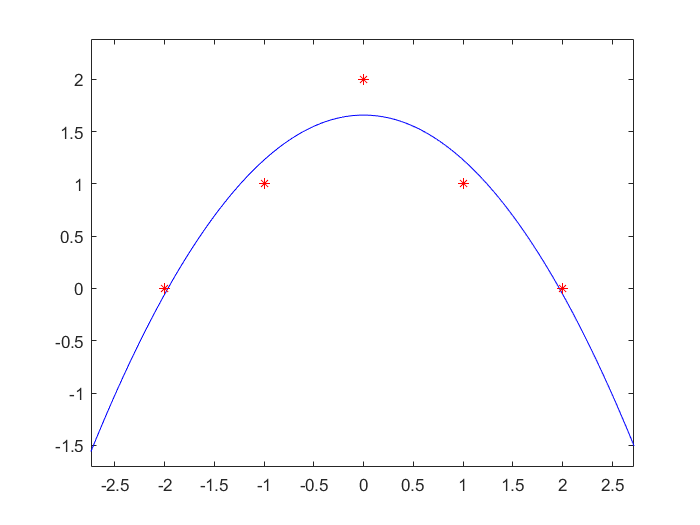
\includegraphics[width=0.7\columnwidth]{figures/lspoly.png}
		\caption{观测数据及根据其拟合的二次多项式}
		\label{fig:figure1}
	\end{center}
\end{figure}
\end{document}
